\section{Tasks}
Existing ``macro-scale'' methods can determine if an intervention has a significant influence over our target behavior, but they do not give much insight into how the event has an effect over time.
The dynamic response to the intervention has only recently become available for study thanks to increasingly ubiquitous wearable sensor technology, and so conventional methods have dealt with low-frequency outcome measures with clever study design.
Now that measurement of outcomes can be performed at much higher frequencies, methods which leverage this additional information should be adopted.

The dynamic response of the targeted behavior leading up to and following the event tells us much more about how this effect begins and fades over time.
A deeper look into the shape of the signal following our event may even reveal a significant effect overlooked by our previous analysis, and much more quantitative behavioral models become possible.

From the goals outlined in the design guidelines section, we have identified several key tasks which a researcher might undertake and present visuals to address these tasks.

\subsection{Highlighting Event Dynamics}
The dynamics surrounding a particular event are most commonly shown using a time series.
The instance or span of the event is marked on the time-axis and the value of the behavioral measure (physical activity in this case) is encoded in the height at each point in time.
We can describe several idealized intervention types based on behavioral theory using this common visualization paradigm.

\begin{figure}
\centering
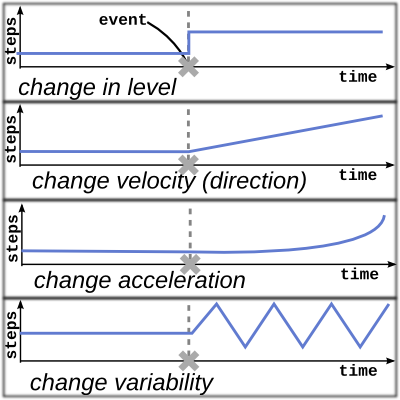
\includegraphics[width=0.6\columnwidth]{./img/exampleDynamicSignals.png}
\caption{Theoretical responses to an intervention (adapted from \cite{glass1975}).}
\label{fig:exampleSignals}
\end{figure}

Figure \ref{fig:exampleSignals} shows the case where an event instantaneously causes permanent change in the target behavior, but in the many cases the intervention will have a temporary effect on the target behavior and will have some delay before setting in.

\begin{figure}
\centering
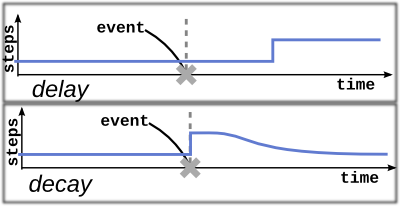
\includegraphics[width=0.6\columnwidth]{./img/exampleDynamicComplications.png}
\caption{Level-change responses with delay and decay (adapted from \cite{glass1975}).}
\label{fig:exampleComplications}
\end{figure}

These intervention response dynamics as shown in figure \ref{fig:exampleComplications} are critically important for just-in-time adaptive intervention developers, but are largely unaddressed in current theory.

\subsection{Event-time Alignment}

\begin{figure}
\centering
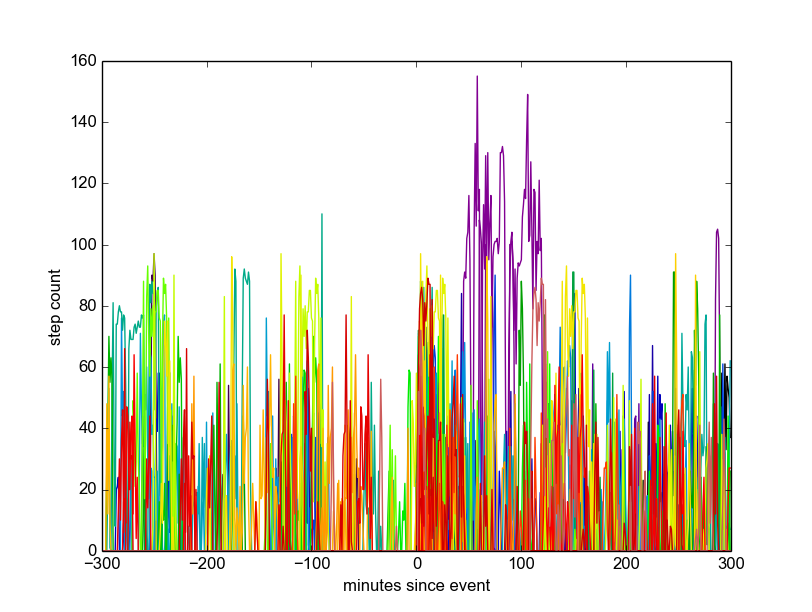
\includegraphics[width=0.9\columnwidth]{./img/perfect_intervention_individual_events.png}
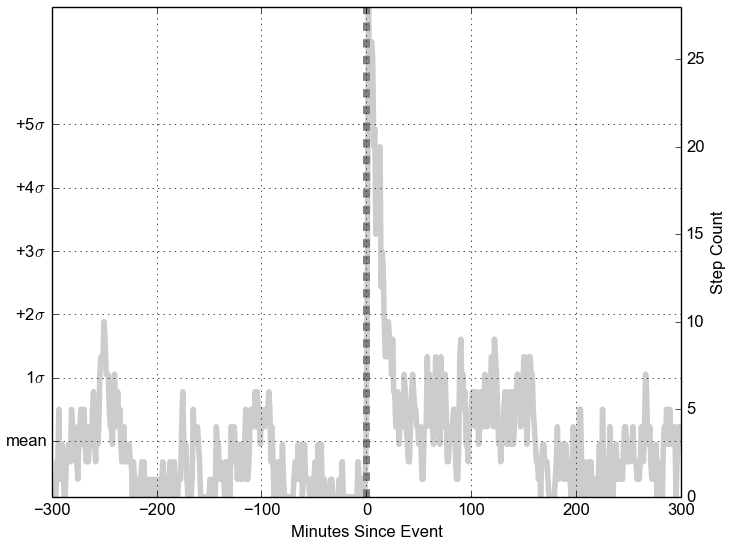
\includegraphics[width=0.9\columnwidth]{./img/perfect_intervention.png}
\caption{Comparison of all event responses (top) to average response (bottom) surrounding the control dataset intervention.}
\label{fig:interventionAverage}
\end{figure}

Figures \ref{fig:exampleSignals} and \ref{fig:exampleComplications} give us sense of what an intervention should look like, but in reality individual variations in context completely mask the often small effect of an intervention (see Figure \ref{fig:interventionAverage} (top)).
This is a familiar problem with a familiar solution.
By time-shifting our data view so that each intervention event falls at t=0 in a time-series, we can average the series together in order to identify effects which are common between all events.
Aggregated measurements surrounding each event begin to give a better picture of the latency and delay of the response.

This approach can be taken for all events in one subject's time series to characterize that subject, or can be applied across subjects to characterize a more generalized response to the intervention.

Figure \ref{fig:interventionAverage} makes clear the value of this method for drawing general conclusions from a set of seemingly random data.
When looking at all events individually (figure \ref{fig:interventionAverage} top), it is difficult to spot any pattern in the series.
One notable event seems to stand above the rest from 20-60min following the intervention, and a cursory glance at this visual might lead one to believe that this intervention was only effective in that one instance.
When averaging across all event responses, however, a clear, significant response is evident (figure \ref{fig:interventionAverage} bottom).

As expected, figure \ref{fig:interventionAverage} shows the control intervention to be quite effective at increasing the step count.
The additional y-axis showing the mean and standard deviation of the series is included to give an increased sense of the significance of this effect relative to data which may be out of frame.
In addition to the nearly immediate response, a longer-lasting effect reaching out to approximately 180m after the event seems to be boosting step count, though the all-events view in figure \ref{fig:interventionAverage} as well as the stacked-events display in Figure 1 reveal that there are two events which may be the the cause.
Though the average line-graph makes spotting effects easy, we must be wary of outlying events or participants which can skew the average.
This danger can be sometimes mitigated through use of median in place of mean, but since step-count does not obey a normal distribution (0 values are almost always modal), that approach does not work well in this case.

\subsection{Stacking}
To address the shortcomings of the aforementioned average-line shown in figure \ref{fig:interventionAverage}, individual events can be shown on the graph and stacked.
This yields the same shape, and the y-axis can be easily normalized to match our average series by dividing by the number of events.
While still “averaging out” random contextual influences, this visual also provides indication that the average result is not due to one outlier event, enables easy spotting of missing data or faulty sensors, and gives some indication of the number of events considered.
For an n-of-one dataset such as the control dataset, events can be graphed with a unique color.
In figure 1, event colors are chosen based on the order in which they were observed.
Color mapping of events can also be used to visually group events based on time of day, location of the event, or participant.

\begin{figure}
\centering
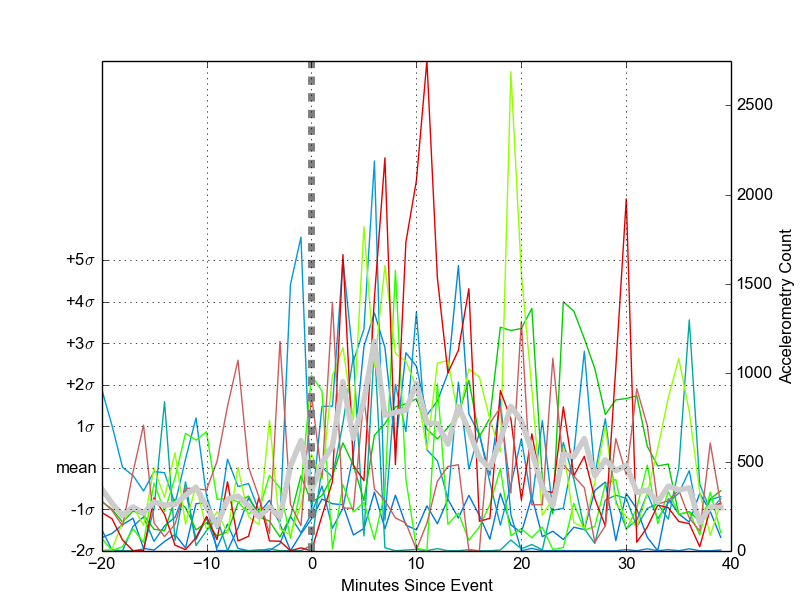
\includegraphics[width=0.9\columnwidth]{./img/knowMe_60m_lines.png}
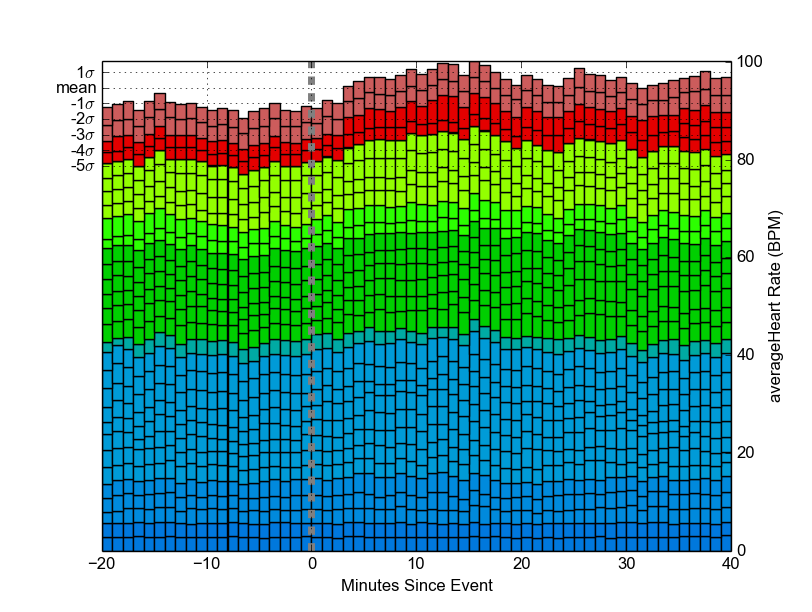
\includegraphics[width=0.9\columnwidth]{./img/knowMe_60m_bars.png}
\caption{Comparison of knowMe average lines and stacked bars.}
\label{fig:knowMeCompare}
\end{figure}

Figure \ref{fig:knowMeCompare} shows the difference between a plot of various average response lines and the stacked area plot.
The thin lines in figure \ref{fig:knowMeCompare} (top) represent the response of each participant to the event averaged across all events for that participant.
The thick line shows the average across all participant’s average series.

The stacked bars in figure \ref{fig:knowMeCompare} (bottom) are colored by participant ID, and each represent one unique event - stacked in order of event incidence.
This allows researchers to search for both participant outliers within the set as well as event outliers within each participant.

The linegraph allows for identification of unqiue individuals (such as red, light blue TODO: mark these and reference by marker not color), but the stackplot better highlights the overall effect and also shows the number of events considered.
Another key difference between these two approaches is the proporitonate weighting of subjects into the global effect display.
The line-graph approach considers each subject equally regarless of the number of events recorded of that subject, whereas the stackplot considers the events equally and thus each subject's contribution is weighted by the number of events recorded.

\begin{equation}
	\bar{y}(t) = \frac{1}{N} \sum\limits_{i=1}^N y_i(t)
	\label{eq:barAvg}
\end{equation}

\begin{equation}
	\bar{y}(t) = \frac{1}{P} \sum\limits_{p=1}^P \frac{1}{n_p} \sum\limits{i=1}^n_p y_{i,p}(t)
	\label{eq:lineAvg}
\end{equation}
	
Equations (\ref{eq:barAvg}) and (\ref{eq:lineAvg}) shows the difference in aggregation methods for line vs stacked views where $N$ is the total number of events across all participants, $P$ is the number of participants, $n_p$ represents the number of events for subject $p$,  $y_i$ represents the time series for event $i$, and $y_{i,p}$ represents the time series for subject $p$'s event $i$.
Aggretating data via method (\ref{eq:lineAvg}) does a better job to ensure that one participant does not skew results, but can give too much weight to data from a participant with few events.

Figure \ref{fig:knowMeCompare} shows an increase in heart rate (TODO: use a different measure. which one?) following the delivery of a physical-activity-suggesting sms message.
Though the behavioral measure differs greatly from that used in the control dataset and \ref{fig:interventionAverage}, a comparison of the y-values in terms of standard deviation also reveals that this effect is less extreme than what we observe in the control intervention.

The deviation from the mean as measured relative to the standard deviation gives a sense of how unlikely the signal is to be a random artifact, but methods for evaluating the statistical likelihood of observing a particular shape are not covered here.

\subsection{Characterize Intervention Delivery Context}
In some cases introducing a “control event” against which to compare the experimental event can help isolate the intervention from the context in which it is delivered.
For instance, an intervention delivered on a mobile device is always delivered within the context of phone interaction.
That is, the user is always using the phone when the intervention is delivered.
It is possible that "using the phone" has it's own unique effect on the behavioral measure.
Thus, using "phone use" events as a baseline against which to compare "phone use and intervention delivery" strengthens the chance that the observed effect is a result of the intervention itself and not the result of frequently concurrent contextual forces. 
For example, by looking at all times the phone was viewed in the mAvatar dataset, we can characterize the average context of phone use.

\begin{figure}
\centering
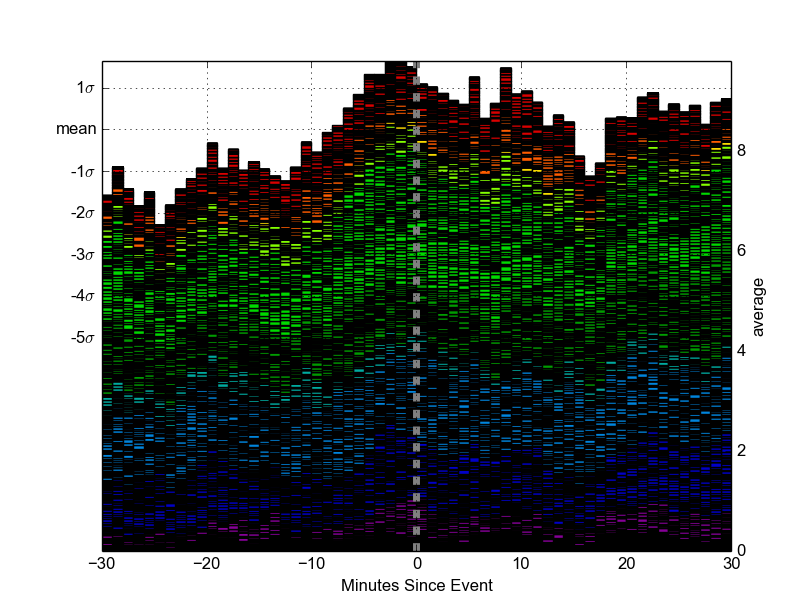
\includegraphics[width=0.9\columnwidth]{./img/mAvatarViews_1673_wOverlap.png}
\caption{Stackplot of step counts in the 30 minutes surrounding 1673 phone-view events from the mAvatar dataset.}
\label{fig:mAvatarPhoneContext}
\end{figure}

In figure \ref{fig:mAvatarPhoneContext}, we see a notable increase in steps leading up to phone usage.
It is possible that this increase - though it prempts avatar viewing - is indeed caused by the avatar.
Consider, for instance, the unanimously reported case of subjects viewing the phone with the explicit purpose of seeing how the avatar would be affected by their behavior.
Thus we should perhaps expect to see a peak in PA driven by the desire to illicit a response from the avatar, which is viewed only a few minutes later.
This interpretation is quite speculative and other features of figure \ref{fig:mAvatarPhoneContext} are not so easily explained.
It is clear, however, that this is not a flat baseline that we may expect to find on average, and exploration of dynamics surrounding the active and sedentary avatar viewings ought to subtract this baseline to account for the overlapping of this context-driven (rather than event-driven) signal.
In the specific case of the mAvatar dataset, however, we may utilize a direct comparison between events, rather than a comparison of each event vs the baseline.

/comment{
The results of this analysis were not interesting; the control data looks the same when processed this way

Using the control dataset as an example, random points in time when the subject was at his desk can serve as the control event against which to compare the experimental "intervention" event.

To represent a difference between two intervention effect time series visually we return to the use of line averages due to the confounding nature of negatively-valued bars in stacked graphs.

TODO: fig line graph of controlData avg(intervention)-avg(control)
}

\subsection{Comparing Event Types}
Aforementioned methods used to provide a contextual baseline of comparison for events can also be applied to allow for a comparison between two event types.
By treating one event as the baseline, differences between the events can be visualized.
Using this paradigm, nearly equivalent event responses will have a near-zero difference.
Positively-valued areas of the resulting chart indicate times when the "experimental event" had a greater positive effect on the target measure, or, conversely, that the "control event" had a greater negative effect on the target measure.


The mAvatar dataset contains two types of intervention which may be interesting to compare: 1) active-avatar viewing, 2) sedentary-avatar viewing.
In this case, the two event types are theoretically opposite in effect, meaning that the sedentary-avatar effect should resemble a mirrored version of the active-avatar effect.
Thus, the difference should accentuate the intervention's effect signature and better isolate the behavioral response from noisy data.

\begin{figure}
\centering
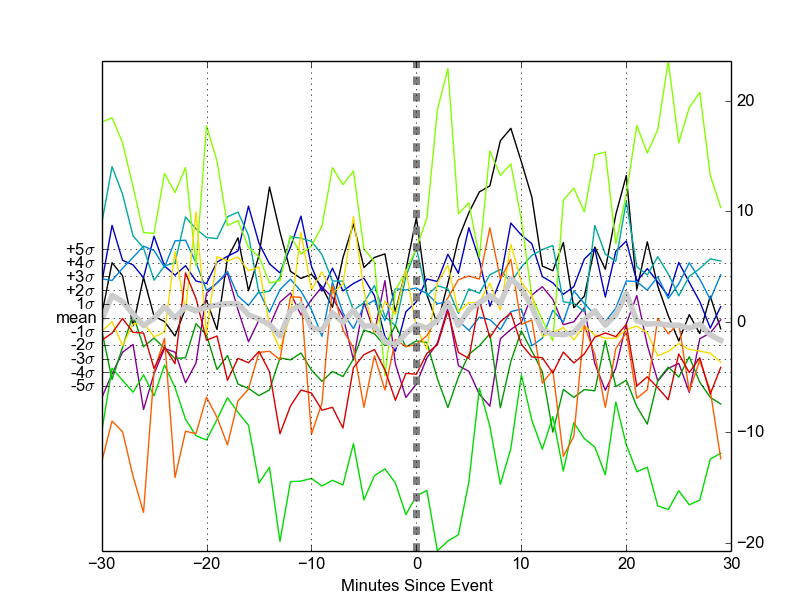
\includegraphics[width=0.9\columnwidth]{./img/mAvatar_difference_events.png}
\caption{Active-event series average minus sedentary-event series average. (average shown as bold)}
\label{fig:mAvatarDifference}
\end{figure}

Even with two oppositely-polarized events figure \ref{fig:mAvatarDifference} fails to show the dramatic effect a researcher might hope for on average.
The lack of observed effect indicates that the intervention had no effect on average.
In this case, researchers attribute the apparent lack of effect to an ambiguity in study design which led to two opposing conditions: 1) subjects respond positively to physically-active avatars via the Proteus Effect \cite{???} 2) subjects respond negatively to physically-active avatars via falsely perceived biofeedback.

Figure \ref{fig:mAvatarDifference} suggests this subgrouping within the data in the individual participant series.

TODO: talk more about the subgroups (+ response vs -response), label the series.

\comment{
\section{Domain Expert Feedback}
TODO: what do domain experts think about these methods (Donna? Eric?)
}
